\documentclass[a4paper,11pt]{article}
\usepackage{amsmath,amsthm,amsfonts,amssymb,amscd,amstext,vmargin,graphics,graphicx,tabularx,multicol} 
\usepackage[francais]{babel}
\usepackage[utf8]{inputenc}  
\usepackage[T1]{fontenc} 
\usepackage{pstricks-add,tikz,tkz-tab,variations}
\usepackage[autolanguage,np]{numprint} 

\setmarginsrb{1.5cm}{0.5cm}{1cm}{0.5cm}{0cm}{0cm}{0cm}{0cm} %Gauche, haut, droite, haut
\newcounter{numexo}
\newcommand{\exo}[1]{\stepcounter{numexo}\noindent{\bf \underline{Exercice~\thenumexo}}}
\reversemarginpar


\newcounter{enumtabi}
\newcounter{enumtaba}
\newcommand{\q}{\stepcounter{enumtabi} \theenumtabi.  }
\newcommand{\qa}{\stepcounter{enumtaba} (\alph{enumtaba}) }
\newcommand{\initq}{\setcounter{enumtabi}{0}}
\newcommand{\initqa}{\setcounter{enumtaba}{0}}

\newcommand{\be}{\begin{enumerate}}
\newcommand{\ee}{\end{enumerate}}
\newcommand{\bi}{\begin{itemize}}
\newcommand{\ei}{\end{itemize}}
\newcommand{\bp}{\begin{pspicture*}}
\newcommand{\ep}{\end{pspicture*}}
\newcommand{\bt}{\begin{tabular}}
\newcommand{\et}{\end{tabular}}
\renewcommand{\tabularxcolumn}[1]{>{\centering}m{#1}} %(colonne m{} centrée, au lieu de p par défault) 
\newcommand{\tnl}{\tabularnewline}

\newcommand{\bmul}[1]{\begin{multicols}{#1}}
\newcommand{\emul}{\end{multicols}}

\newcommand{\trait}{\noindent \rule{\linewidth}{0.2mm}}
\newcommand{\hs}[1]{\hspace{#1}}
\newcommand{\vs}[1]{\vspace{#1}}

\newcommand{\N}{\mathbb{N}}
\newcommand{\Z}{\mathbb{Z}}
\newcommand{\R}{\mathbb{R}}
\newcommand{\C}{\mathbb{C}}
\newcommand{\Dcal}{\mathcal{D}}
\newcommand{\Ccal}{\mathcal{C}}
\newcommand{\mc}{\mathcal}

\newcommand{\vect}[1]{\overrightarrow{#1}}
\newcommand{\ds}{\displaystyle}
\newcommand{\eq}{\quad \Leftrightarrow \quad}
\newcommand{\vecti}{\vec{\imath}}
\newcommand{\vectj}{\vec{\jmath}}
\newcommand{\Oij}{(O;\vec{\imath}, \vec{\jmath})}
\newcommand{\OIJ}{(O;I,J)}




\newcommand{\reponse}[1][1]{%
\multido{}{#1}{\makebox[\linewidth]{\rule[0pt]{0pt}{20pt}\dotfill}
}}

\newcommand{\titre}[5] 
% #1: titre #2: haut gauche #3: bas gauche #4: haut droite #5: bas droite
{
\noindent #2 \hfill #4 \\
#3 \hfill #5

\vspace{-1.6cm}

\begin{center}\rule{6cm}{0.5mm}\end{center}
\vspace{0.2cm}
\begin{center}{\large{\textbf{#1}}}\end{center}
\begin{center}\rule{6cm}{0.5mm}\end{center}
}



\begin{document}
\pagestyle{empty}
\titre{Chapitre 6 : Écritures fractionnaires}{}{}{}{}

\vspace*{1cm}

\begin{center}
{\Large \textbf{Niveau 1 :}}
\end{center}

\vspace*{1cm}

$\rightarrow$ \textbf{Fractions et partage}\\

\vspace*{0.5cm}



\exo \\  Trois élèves ont colorié le tiers d'un carré. Quel élève a raison ?\\

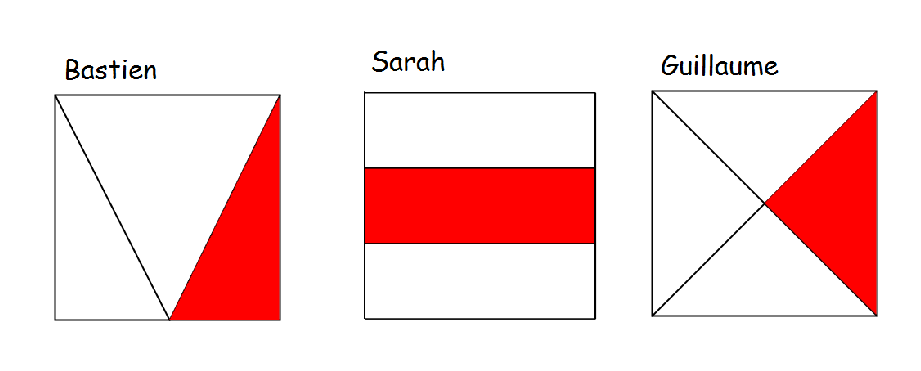
\includegraphics[scale=0.65]{fraction2.eps} \\

\noindent \reponse[1]\\

 \exo \\ Exprimer à l'aide d'une fraction, l'aire totale qui correspond à la partie est colorée.\\
 
 \includegraphics[scale=0.65]{fraction4.eps} \\
 
 \vspace*{1cm}

$\rightarrow$ \textbf{Fractions et demi-droite graduée}\\

\vspace*{0.5cm}

\exo \\ Écrire les abscisses des points E, F et G sous forme de fractions.\\

\includegraphics[scale=1]{abscisse1.eps} \\

E( . . . ) \hspace*{1.5cm} F( . . . ) \hspace*{1.5cm}  G( . . . )\\


\exo \\ Retrouver les noms des points qui correspondent aux abscisses ci-dessous.\\

\includegraphics[scale=0.8]{abscisse11.eps} \\

. . . ( $\dfrac{9}{4}$ ) \hspace*{1.5cm} . . . ( $\dfrac{1}{4}$ ) \hspace*{1.5cm}  . . . ( $\dfrac{12}{4}=3$ ) \hspace*{1.5cm}  . . . ( $\dfrac{5}{4}$ )\\

\vspace*{1cm}

$\rightarrow$ \textbf{Fraction d'une quantité, problèmes}\\


\vspace*{0.5cm}

\exo \\ Énigmes \\

\initqa \qa Mon numérateur est le dénominateur de $\dfrac{12}{29}$ et mon dénominateur est le numérateur de $\dfrac{41}{16}$.\\
\reponse[2]\\

\qa Mon numérateur est le double de celui de $\dfrac{7}{11}$ et mon dénominateur est le tiers de $\dfrac{18}{36}$.\\
\reponse[2]\\

\exo \\ Écrire le calcul qui correspond à chaque phrase sans effectuer le calcul.\\

\initqa \qa Le quart de 100 : . . . . . . . . . . . . . . . . . . . .\\


 \qa Les sept tiers de 126 : . . . . . . . . . . . . . . . . . . . .\\

 
  \qa Les trois quart de 280 : . . . . . . . . . . . . . . . . . . . .\\

  
   \qa Les cinq demis de 30 : . . . . . . . . . . . . . . . . . . . .\\

   
  \vspace*{1cm}

$\rightarrow$ \textbf{Écritures fractionnaires égales}\\

\vspace*{0.5cm}


\exo \\ Compléter avec les nombres qui conviennent.\\

\includegraphics[scale=1]{egal2.eps}  \hspace*{0.6cm} \includegraphics[scale=0.5]{egal3.eps}\\
     
\vspace*{1cm}

$\rightarrow$ \textbf{Simplification de fractions}\\

\vspace*{0.5cm}


\exo \\ Repérer et réécrire les fractions qui sont irréductibles, c'est-à-dire non simplifiables.\\

\includegraphics[scale=0.7]{simplifier1.eps} \\

Réponse :\\
\noindent \reponse[2]\\


\exo \\ Simplifier les fractions par 2 comme dans l'exemple ci-dessous.\\

\begin{center}
$\dfrac{26}{10} = \dfrac{26 \div 2}{10 \div 2} =$ \fbox{$\dfrac{13}{5}$}
\end{center}

\initqa \qa $\dfrac{6}{10} = \dfrac{6 \div 2}{10 \div 2} = \dfrac{....}{....}$\\

\qa $\dfrac{14}{16}= \dfrac{.... \div ....}{.... \div ....}=$\\


\qa $\dfrac{22}{8}= \dfrac{.... \div ....}{.... \div ....}=$\\


\qa $\dfrac{50}{64}= \dfrac{.... \div ....}{.... \div ....}=$\\


\exo \\ Simplifier les fractions par 3 comme dans l'exemple ci-dessous.\\

\begin{center}
$\dfrac{21}{111} = \dfrac{21 \div 3}{111 \div 3} =$ \fbox{$\dfrac{7}{37}$}
\end{center}

\initqa \qa $\dfrac{27}{12} = \dfrac{27 \div 3}{12 \div 3} = \dfrac{....}{....}$\\

\qa $\dfrac{63}{18}= \dfrac{.... \div ....}{.... \div ....}=$\\


\qa $\dfrac{33}{24}= \dfrac{.... \div ....}{.... \div ....}=$\\


\qa $\dfrac{3}{6}= \dfrac{.... \div ....}{.... \div ....}=$\\

\exo \\ Parmi les fractions suivantes, quelles sont les fractions qui peuvent être encore simplifiées ?\\
\begin{center}
$\dfrac{45}{105}$ \hspace*{1.5cm}  $\dfrac{140}{90}$ \hspace*{1.5cm}   $\dfrac{97}{3}$ \hspace*{1.5cm}  $\dfrac{123}{48}$ \hspace*{1.5cm} $\dfrac{25}{46}$ \hspace*{1.5cm}  $\dfrac{124}{712}$
\end{center}
\reponse[2]\\

\exo \\ Parmi les écritures fractionnaires suivantes, quelles sont celles qui sont des fractions ?\\
\begin{center}
$\dfrac{40}{100}$ \hspace*{1.5cm}  $\dfrac{2,8}{1,6}$ \hspace*{1.5cm}   $\dfrac{1256}{7}$ \hspace*{1.5cm}  $\dfrac{0,125}{10}$ \hspace*{1.5cm} $\dfrac{45}{11,7}$ \hspace*{1.5cm}  $\dfrac{0,1}{0,2}$
\end{center}
\reponse[2]\\

\vspace*{0.5cm}

\begin{center}
{\Large \textbf{Niveau 2 :}}
\end{center}




\vspace*{1cm}

$\rightarrow$ \textbf{Fractions et partage}\\

\vspace*{0.5cm}

\exo \\ Citer les figures où le quart de la surface a  bien été coloriée.\\

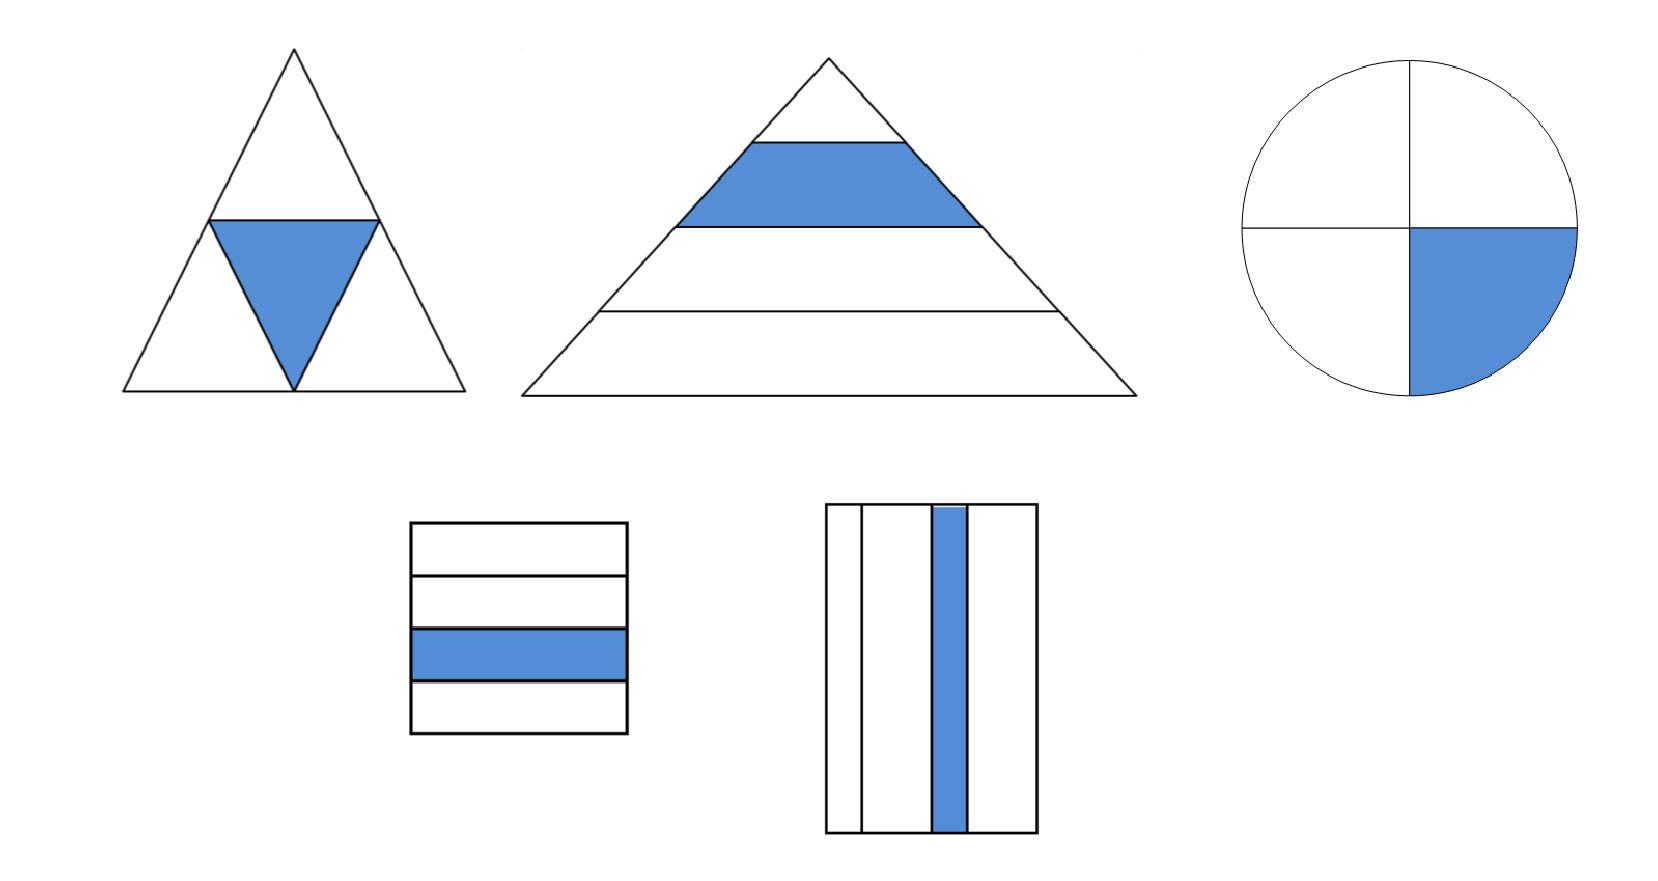
\includegraphics[scale=0.6]{fraction3.eps} \\

\noindent \reponse[1]\\

\vspace*{0.5cm}

\exo \\ Exprimer à l'aide d'une fraction, l'aire totale qui correspond à la partie est colorée.\\
 
 \includegraphics[scale=0.65]{fraction5.eps} \\
 
 
  \vspace*{1cm}

$\rightarrow$ \textbf{Fractions et demi-droite graduée}\\

\vspace*{0.5cm}

\exo \\ Écrire les abscisses des points E, F et G sous forme de fractions.\\

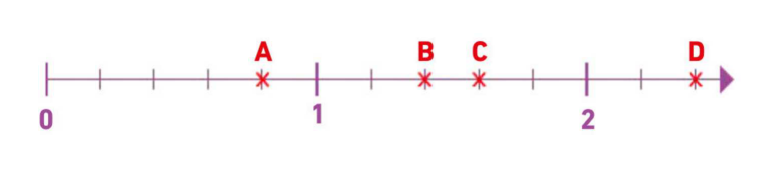
\includegraphics[scale=1]{abscisse2.eps} \\

A( . . . ) \hspace*{1.5cm} B( . . . ) \hspace*{1.5cm}  C( . . . ) \hspace*{1.5cm}  D( . . . )\\

\exo \\ Retrouver les noms des points qui correspondent aux abscisses ci-dessous.\\

\includegraphics[scale=0.8]{fraction22.eps} \\

. . . ( $\dfrac{9}{3}$ ) \hspace*{1.5cm} . . . ( $\dfrac{2}{3}$ ) \hspace*{1.5cm}  . . . ( $\dfrac{13}{3}$ ) \hspace*{1.5cm}  . . . ( $\dfrac{7}{3}$ )\\



\vspace*{1cm}

$\rightarrow$ \textbf{Fraction d'une quantité, problèmes}\\


\vspace*{0.5cm}


\exo \\ Écrire les calculs  correspondant à chaque phrase et les effectuer.\\

\initqa \qa Le quart de 32 : . . . . . . . . . . . . . . . . . . . .\\

\qa Les deux tiers de 45: . . . . . . . . . . . . . . . . . . . .\\

\qa Les trois demis de 16 : . . . . . . . . . . . . . . . . . . . .\\

\qa Le tiers de 33 : . . . . . . . . . . . . . . . . . . . .\\


\exo \\ Il y a au total 21 étoiles.\\

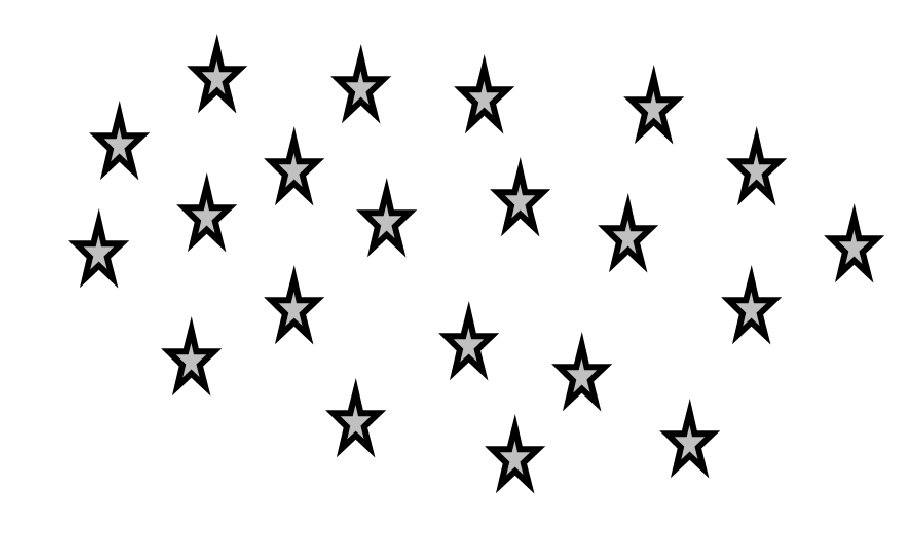
\includegraphics[scale=1]{pb1.eps} \\

On souhaite prendre $\dfrac{1}{3}$ de toutes les étoiles. Combien d'étoiles cela représente-t-il?\\
\reponse[2]\\

\exo \\ Il y a au total 21 étoiles.\\

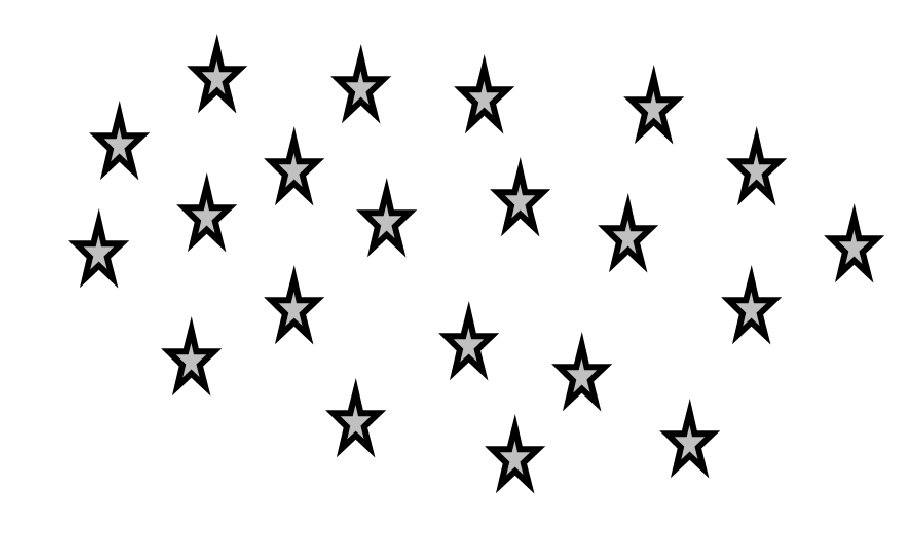
\includegraphics[scale=1]{pb1.eps} \\

On souhaite prendre $\dfrac{2}{7}$ de toutes les étoiles. Combien d'étoiles cela représente-t-il?\\
\reponse[2]\\

\vspace*{1cm}

$\rightarrow$ \textbf{Écritures fractionnaires égales}\\

\vspace*{0.5cm}


\exo \\ Compléter les égalités suivantes comme sur le modèle ci-dessous.\\

\begin{center}
\includegraphics[scale=0.85]{egal1.eps} 
\end{center}

\initqa \qa $\dfrac{1}{4} = \dfrac{....}{20}$\\

 \qa $\dfrac{7}{8} = \dfrac{21}{....}$\\
 
  \qa $\dfrac{3}{5} = \dfrac{....}{45}$\\
  
   \qa $\dfrac{10}{6} = \dfrac{50}{....}$\\
   
    \qa $\dfrac{2}{7} = \dfrac{....}{77}$\\
    
     \qa $ 3 = \dfrac{3}{1} = \dfrac{....}{15}$\\



\vspace*{1cm}

$\rightarrow$ \textbf{Simplification de fractions}\\

\vspace*{0.5cm}



\exo \\ Simplifier les fractions par 5 comme dans l'exemple ci-dessous.\\

\begin{center}
$\dfrac{70}{25} = \dfrac{70 \div 5}{25 \div 5} =$ \fbox{$\dfrac{14}{5}$}
\end{center}

\initqa \qa $\dfrac{25}{45} = \dfrac{25 \div 5}{45 \div 5} = \dfrac{....}{....}$\\

\qa $\dfrac{30}{55}= \dfrac{.... \div ....}{.... \div ....}=$\\


\qa $\dfrac{20}{5}= \dfrac{.... \div ....}{.... \div ....}=$\\


\qa $\dfrac{10}{65}= \dfrac{.... \div ....}{.... \div ....}=$\\



\exo \\ Simplifier les fractions par 7 comme dans l'exemple ci-dessous.\\

\begin{center}
$\dfrac{56}{21} = \dfrac{56 \div 7}{21 \div 7} =$ \fbox{$\dfrac{8}{3}$}
\end{center}

\initqa \qa $\dfrac{14}{49} = \dfrac{14 \div 7}{49 \div 7} = \dfrac{....}{....}$\\

\qa $\dfrac{7}{28}= \dfrac{.... \div ....}{.... \div ....}=$\\


\qa $\dfrac{35}{42}= \dfrac{.... \div ....}{.... \div ....}=$\\


\qa $\dfrac{63}{84}= \dfrac{.... \div ....}{.... \div ....}=$\\


\exo \\ Cliquer sur la bonne réponse.\\

\renewcommand{\arraystretch}{3}

\begin{tabular}{|c|c|c|c|c|}
\hline 
\textbf{Questions} & \textbf{a} & \textbf{b} & \textbf{c} & \textbf{d} \\ 
\hline 
$\dfrac{22}{16}=$ & $\dfrac{2}{6}$ & $\dfrac{11}{16}$ & $\dfrac{1}{2}$ & $\dfrac{11}{8}$ \\ 
\hline 
$\dfrac{350}{150}=$ & $\dfrac{2}{5}$ & $\dfrac{7}{3}$ & $\dfrac{7}{15}$ & $\dfrac{3}{15}$ \\
\hline 
$\dfrac{6}{12}=$ & $\dfrac{6}{3}$ & $\dfrac{1}{2}$ & $\dfrac{3}{4}$ & $\dfrac{2}{3}$ \\ 
\hline 
$\dfrac{8}{20}=$ & $\dfrac{4}{5}$ & $\dfrac{1}{5}$ & $\dfrac{2}{5}$ & $\dfrac{2}{10}$ \\
\hline 
\end{tabular} 

\begin{center}
{\Large \textbf{Niveau 3 :}}
\end{center}

\vspace*{1cm}


\vspace*{1cm}

$\rightarrow$ \textbf{Fractions et partage}\\

\vspace*{0.5cm}



\vspace*{0.5cm}

\exo \\ Exprimer à l'aide d'une fraction, l'aire totale qui correspond à la partie est colorée.\\
 
 \includegraphics[scale=0.65]{fraction6.eps} \\

\vspace*{0.5cm}


 \vspace*{1cm}

$\rightarrow$ \textbf{Fractions et demi-droite graduée}\\

\vspace*{0.5cm}

\exo \\ Écrire les abscisses des points E, F et G sous forme de fractions.\\

\includegraphics[scale=0.9]{abscisse3.eps} \\

G( . . . ) \hspace*{1.5cm} H( . . . ) \hspace*{1.5cm}  J( . . . )\\



\exo \\ Retrouver les noms des points qui correspondent aux abscisses ci-dessous.\\

\includegraphics[scale=0.8]{abscisse33.eps} \\

. . . ( $\dfrac{5}{4}$ ) \hspace*{1.5cm} . . . ( $\dfrac{7}{2}$ ) \hspace*{1.5cm}  . . . ( $\dfrac{9}{4}$ ) \hspace*{1.5cm}  . . . ( $\dfrac{6}{2}$ )\\


\exo \\ Retrouver les noms des points qui correspondent aux abscisses ci-dessous.\\

\includegraphics[scale=0.8]{abscisse33b.eps} \\

. . . ( $\dfrac{31}{3}$ ) \hspace*{1.5cm} . . . ( $\dfrac{25}{3}$ ) \hspace*{1.5cm}  . . . ( $\dfrac{20}{3}$ ) \hspace*{1.5cm}  . . . ( $\dfrac{28}{3}$ )\\




\vspace*{1cm}

$\rightarrow$ \textbf{Fraction d'une quantité, problèmes}\\


\vspace*{0.5cm}


\exo \\ Calculer les expressions suivantes :\\

\initqa \qa $\dfrac{3}{8}  \times 160$ = . . . . .\\

\qa $\dfrac{7}{5}  \times 200$ = . . . . .\\

\qa $\dfrac{8}{10}  \times 25$ = . . . . .\\

\qa $\dfrac{9}{11}  \times 88$ = . . . . .\\


\exo \\ Calculer les expressions suivantes :\\

\initqa \qa $\dfrac{7}{9}  \times 63$ m = . . . . .\\

\qa $\dfrac{12}{7}  \times 77$ euros = . . . . .\\

\qa $\dfrac{3}{4}  \times 100$ L = . . . . .\\

\qa $\dfrac{5}{8}  \times 64$ g = . . . . .\\

\exo \\ Une plaquette de beurre pèse 500 g. Combien pèse alors une demie plaquette de beurre ?\\

Calculs : \\
\reponse[2]\\

Phrase réponse :\\
\reponse[2]\\

\exo \\ Dans un litre, il y a 1 000 millilitres. Combien il y a-t-il de millilitres dans un quart de litre ?\\

Calculs : \\
\reponse[2]\\

Phrase réponse :\\
\reponse[2]\\


\vspace*{1cm}

$\rightarrow$ \textbf{Écritures fractionnaires égales}\\

\vspace*{0.5cm}


\exo \\ Compléter les égalités suivantes.\\

\bmul{3}

$\dfrac{1}{6}=\dfrac{.....}{30}$\\


$\dfrac{35}{42}=\dfrac{.....}{6}$\\

\columnbreak

$\dfrac{3}{72}=\dfrac{1}{....}$\\

$7 = \dfrac{....}{8}$\\


\columnbreak

$\dfrac{5}{7}=\dfrac{40}{.....}$\\

$\dfrac{11}{12}=\dfrac{.....}{60}$\\



\emul




\exo \\ Dans chaque cas, compléter par le symbole "=" ou "$\neq$".\\

\initqa \qa $\dfrac{2}{3} ..... \dfrac{10}{15}$\\

\qa $\dfrac{11}{12} ..... \dfrac{120}{110}$\\

\qa $\dfrac{3}{7} ..... \dfrac{24}{63}$\\

\qa $\dfrac{28}{35} ..... \dfrac{4}{6}$\\	



\vspace*{1cm}

$\rightarrow$ \textbf{Simplification de fractions}\\

\vspace*{0.5cm}



\exo \\ Simplifier au maximum les fractions suivantes en utilisant les critères de divisibilité. Vous pouvez faire autant d'étapes que vous le souhaitez. \\

Un exemple :\hspace*{1.5cm} $\dfrac{12}{18} = \dfrac{12 \div 2}{18 \div 2} =  \dfrac{6}{9} =  \dfrac{6 \div 3}{9 \div 3}= $ \fbox{$\dfrac{2}{3}$} ou plus rapide : \hspace*{1.5cm} $\dfrac{12}{18} = \dfrac{12 \div 6}{18 \div 6} = $ \fbox{$\dfrac{2}{3}$}\\


\initqa \qa $\dfrac{28}{36} = \dfrac{.... \div ....}{.... \div ....}=$\\

\qa $\dfrac{25}{125}= \dfrac{.... \div ....}{.... \div ....}=$\\


\qa $\dfrac{20}{160}= \dfrac{.... \div ....}{.... \div ....}=$\\


\qa $\dfrac{60}{144}= \dfrac{.... \div ....}{.... \div ....}=$\\






\begin{center}
{\Large \textbf{Niveau 4:}}
\end{center}

\vspace*{1cm}



$\rightarrow$ \textbf{Fractions et partage}\\

\vspace*{0.5cm}



\exo \\ Exprimer à l'aide d'une fraction, l'aire totale qui correspond à la partie est colorée.\\
 
 \includegraphics[scale=0.65]{fraction7.eps} \\

\vspace*{0.5cm}

\vspace*{1cm}

$\rightarrow$ \textbf{Fractions et demi-droite graduée}\\

\vspace*{0.5cm}

\exo \\ Écrire les abscisses des points E, F et G sous forme de fractions.\\

\includegraphics[scale=0.9]{abscisse4.eps} \\

G( . . . ) \hspace*{1.5cm} H( . . . ) \hspace*{1.5cm}  J( . . . )  \hspace*{1.5cm}  K( . . . )\\


\exo \\ Retrouver les noms des points qui correspondent aux abscisses ci-dessous.\\

\includegraphics[scale=0.8]{abscisse44.eps} \\

. . . ( $\dfrac{2}{6}$ ) \hspace*{1.5cm} . . . ( $\dfrac{5}{3}$ ) \hspace*{1.5cm}  . . . ( $\dfrac{7}{6}$ ) \hspace*{1.5cm}  . . . ( $\dfrac{3}{2}$ )\\


\exo \\ Retrouver les noms des points qui correspondent aux abscisses ci-dessous.\\

\includegraphics[scale=0.8]{abscisse44b.eps} \\

. . . ( $\dfrac{8}{6}$ ) \hspace*{1.5cm} . . . ( $\dfrac{1}{3}$ ) \hspace*{1.5cm}  . . . ( $\dfrac{5}{3}$ ) \hspace*{1.5cm}  . . . ( $\dfrac{13}{12}$ )\\


\vspace*{1cm}

$\rightarrow$ \textbf{Fraction d'une quantité, problèmes}\\


\vspace*{0.5cm}


\exo \\ Parmi  deux  classes  de  6ème  (c’est-à-dire  48  élèves), $\dfrac{3}{4}$   des  élèves  vont  faire  du  ski  nautique  à  Noeud-les-Mines. Les  $\dfrac{5}{6}$ des élèves restants vont monter à cheval. \\ 

 Quel est le nombre d'élèves qui monteront à cheval ? \\

Calculs : \\
\reponse[2]\\

Phrase réponse :\\
\reponse[2]\\


 
 

\exo \\ Pour l'anniversaire de Mélanie, ses amis ont acheté 51 bouteilles de jus de fruits. Avant la première danse, ils ont bu $\dfrac{3}{17}$ des bouteilles de jus ; avant la deuxième danse, ils ont bu un tiers des bouteilles restantes.\\

 Combien de bouteilles de jus ont-ils bu avant la première danse ?\\

Calculs : \\
\reponse[2]\\

Phrase réponse :\\
\reponse[2]\\


\exo \\ Paul achète pour sa mère un bouquet de 48 fleurs. Le tiers d'entre elles sont des roses. Les $\dfrac{3}{8}$ du reste sont des mimosas. \\

Combien y a-t-il de mimosas dans le bouquet?\\

Calculs : \\
\reponse[2]\\

Phrase réponse :\\
\reponse[2]\\



\vspace*{1cm}

$\rightarrow$ \textbf{Écritures fractionnaires égales}\\

\vspace*{0.5cm}




\exo \\ Compléter les égalités suivantes :\\

\bmul{3}

{\Large $\dfrac{10}{6} = \dfrac{....}{3} = \dfrac{25}{....}$}\\




\columnbreak

{\Large $\dfrac{45}{60} = \dfrac{3}{....} = \dfrac{....}{28}$}\\






\columnbreak


{\Large $7 = \dfrac{....}{4} = \dfrac{14}{....}$}\\


\emul

\exo \\ Compléter les égalités suivantes :\\

\bmul{3}

{\Large $\dfrac{26}{65} = \dfrac{....}{5} = \dfrac{18}{....}$}\\


\columnbreak

{\Large $\dfrac{27}{36} = \dfrac{3}{....} = \dfrac{....}{40}$}\\

\columnbreak

{\Large $3 = \dfrac{3}{....} = \dfrac{....}{6}$}\\

\emul


\exo \\ Dans la liste de fractions ci-dessous, il y a un intrus. Saurez-vous le repérer ?\\

$\dfrac{800}{1 000}$ \hspace*{1.75cm} $\dfrac{16}{20}$ \hspace*{1.75cm} $\dfrac{4}{5}$ \hspace*{1.75cm} $\dfrac{34}{40}$ \hspace*{1.75cm} $\dfrac{8}{10}$ \\

Réponse : . . . . . . .\\



\vspace*{1cm}

$\rightarrow$ \textbf{Simplification de fractions}\\

\vspace*{0.5cm}



\exo \\ Simplifier au maximum les fractions suivantes en utilisant les critères de divisibilité. Vous pouvez faire autant d'étapes que vous le souhaitez. \\

Un exemple :\hspace*{1.5cm} $\dfrac{12}{18} = \dfrac{12 \div 2}{18 \div 2} =  \dfrac{6}{9} =  \dfrac{6 \div 3}{9 \div 3}= $ \fbox{$\dfrac{2}{3}$} ou plus rapide : \hspace*{1.5cm} $\dfrac{12}{18} = \dfrac{12 \div 6}{18 \div 6} = $ \fbox{$\dfrac{2}{3}$}\\


\initqa \qa $\dfrac{750}{240} = \dfrac{.... \div ....}{.... \div ....}=$\\

\qa $\dfrac{99}{22}= \dfrac{.... \div ....}{.... \div ....}=$\\


\qa $\dfrac{216}{120}= \dfrac{.... \div ....}{.... \div ....}=$\\


\qa $\dfrac{672}{56}= \dfrac{.... \div ....}{.... \div ....}=$\\


\exo \\ Écrire chaque écriture fractionnaire sous la forme d'une fraction.\\

Un exemple :\hspace*{1.5cm} $\dfrac{11,2}{3,9} = \dfrac{11,2 \times 10}{3,9 \times 10} = $ \fbox{$\dfrac{112}{39}$}\\

\initqa \qa $\dfrac{4,7}{0,5} =  \dfrac{.... \times ....}{.... \times ....}= $\\


\qa $\dfrac{3,28}{1,2} =  \dfrac{.... \times ....}{.... \times ....}= $\\

\qa $\dfrac{0,1}{0,03} =  \dfrac{.... \times ....}{.... \times ....}= $\\

\qa $\dfrac{28}{3,9} =  \dfrac{.... \times ....}{.... \times ....}= $\\

\begin{center}
{\Large \textbf{Niveau 5 :}}
\end{center}

\vspace*{1cm}



$\rightarrow$ \textbf{Fractions et partage}\\

\vspace*{0.5cm}



\exo \\ Exprimer à l'aide d'une fraction, l'aire totale qui correspond à la partie est colorée.\\
 
 \includegraphics[scale=0.6]{fraction8.eps} \\
 
 
 
 \vspace*{1cm}

$\rightarrow$ \textbf{Fractions et demi-droite graduée}\\

\vspace*{0.5cm}

\exo \\ Écrire les abscisses des points E, F et G sous forme de fractions.\\

\includegraphics[scale=0.9]{abscisse5.eps} \\

E( . . . ) \hspace*{1.5cm} F( . . . ) \hspace*{1.5cm}  G( . . . )\\


\exo \\ Retrouver les noms des points qui correspondent aux abscisses ci-dessous.\\

\includegraphics[scale=0.8]{abscisse55.eps} \\

. . . ( $\dfrac{9}{12}$ ) \hspace*{1.5cm} . . . ( $\dfrac{3}{2}$ ) \hspace*{1.5cm}  . . . ( $\dfrac{2}{3}$ ) \hspace*{1.5cm}  . . . ( $\dfrac{8}{4}$ )\\

\vspace*{1cm}

$\rightarrow$ \textbf{Fraction d'une quantité, problèmes}\\


\vspace*{0.5cm}

\vspace*{0.5cm}

\exo \\ Parmi  deux  classes  de  6ème  (c’est-à-dire  48  élèves), $\dfrac{3}{4}$   des  élèves  vont  faire  du  ski  nautique  à  Noeud-les-Mines. Les  $\dfrac{5}{6}$ des élèves restants vont monter à cheval. \\ 

 Les élèves qui ne sont ni au ski ni au au cheval sont dispensés de sport. Combien y a-t-il de dispensés ? \\

Calculs : \\
\reponse[2]\\

Phrase réponse :\\
\reponse[2]\\


\exo \\ Pour l'anniversaire de Mélanie, ses amis ont acheté 51 bouteilles de jus de fruits. Avant la première danse, ils ont bu $\dfrac{3}{17}$ des bouteilles de jus ; avant la deuxième danse, ils ont bu un tiers des bouteilles restantes.\\

Combien de bouteilles de jus reste-t-il après la deuxième danse ?\\


Calculs : \\
\reponse[2]\\

Phrase réponse :\\
\reponse[2]\\

\exo \\ L'âne du meunier.\\
  Afin de transporter les grains et la farine, un meunier a acheté deux bêtes de trait : une mule pour 945 f et un âne qu'il a payé les $\dfrac{4}{9}$ du prix de la mule.\\
 
Combien a-t-il dépensé en tout?\\
 
 Calculs : \\
\reponse[2]\\

Phrase réponse :\\
\reponse[2]\\

\exo \\ Paul achète pour sa mère un bouquet de 48 fleurs. Le tiers d'entre elles sont des roses. Les $\dfrac{3}{8}$ du reste sont des mimosas. \\
Les fleurs restantes sont des tulipes.\\

 Une rose coûte 1,22 euros, un mimosa 0,76 euros, une tulipe 0,69 euros.  Quel est le prix du bouquet de fleur ?\\
 
 
Calculs : \\
\reponse[4]\\

Phrase réponse :\\
\reponse[2]\\


\vspace*{1cm}

$\rightarrow$ \textbf{Écritures fractionnaires égales}\\

\vspace*{0.5cm}

\exo \\ Dans la liste de fractions ci-dessous, il y a un intrus. Saurez-vous le repérer ?\\

$\dfrac{12}{16}$ \hspace*{1.75cm} $\dfrac{15}{25}$ \hspace*{1.75cm} $\dfrac{3}{4}$ \hspace*{1.75cm} $\dfrac{75}{100}$ \hspace*{1.75cm} $\dfrac{510}{680}$ \\

Réponse : . . . . . . .\\


\exo \\ Dans la liste de fractions ci-dessous, il y a un intrus. Saurez-vous le repérer ?\\

$\dfrac{91}{115}$ \hspace*{1.75cm} $\dfrac{65}{75}$ \hspace*{1.75cm} $\dfrac{130}{150}$ \hspace*{1.75cm} $\dfrac{13}{15}$ \hspace*{1.75cm} $\dfrac{78}{90}$ \\

Réponse : . . . . . . .\\

\exo \\ Classer dans le tableau les fractions suivantes.\\

$\dfrac{15}{18}$ \hspace*{1.75cm} $\dfrac{6}{9}$ \hspace*{1.75cm} $\dfrac{12}{18}$ \hspace*{1.75cm} $\dfrac{10}{12}$ \hspace*{1.75cm} $\dfrac{21}{28}$ \hspace*{1.75cm} $\dfrac{6}{8}$ \hspace*{1.75cm} $\dfrac{10}{15}$ \hspace*{1.75cm} $\dfrac{20}{24}$ \\

\vspace*{1cm}

\renewcommand{\arraystretch}{3}

\begin{tabular}{|c|p{10cm}|}
\hline 
Fractions égales à $\dfrac{2}{3}$ &  \\ 
\hline 
Fractions égales à $\dfrac{3}{4}$ &  \\ 
\hline 
Fractions égales à $\dfrac{5}{6}$ &  \\ 
\hline 
\end{tabular} 



\vspace*{1cm}

$\rightarrow$ \textbf{Simplification de fractions}\\

\vspace*{0.5cm}



\exo \\ Écrire les écritures fractionnaires sous forme de fractions \textbf{irréductibles}.\\

Un exemple :\hspace*{1.5cm} $\dfrac{11,2}{3,8} = \dfrac{11,2 \times 10}{3,8 \times 10} = \dfrac{112}{38} = \dfrac{112 \div 2}{38 \div 2}$ \fbox{$\dfrac{56}{19}$}\\

\initqa \qa $\dfrac{1,2}{2} =  \dfrac{.... \times ....}{.... \times ....}= $\\


\qa $\dfrac{7,68}{1,4} =  \dfrac{.... \times ....}{.... \times ....}= $\\

\qa $\dfrac{0,96}{0,084} =  \dfrac{.... \times ....}{.... \times ....}= $\\

\qa $\dfrac{10}{2,5} =  \dfrac{.... \times ....}{.... \times ....}= $\\

\exo \\ Message codé\\

\begin{tabular}{|c|c|c|c|c|c|c|c|c|}
\hline 
A & C & I & E & Q & R & S & T & U \\ 
\hline 
$\dfrac{2}{3}$ & $\dfrac{3}{4}$ & $\dfrac{4}{5}$ & $\dfrac{5}{6}$ & $\dfrac{6}{7}$ & $\dfrac{7}{8}$ & $\dfrac{8}{9}$ & $\dfrac{9}{10}$ & $\dfrac{10}{11}$ \\ 
\hline 
\end{tabular} 


Trouver le mot mystère en simplifiant chaque fraction au maximum et en la remplaçant par la lettre correspondante.\\

$\dfrac{405}{450}$ \hspace*{1.5cm} $\dfrac{840}{1050}$ \hspace*{1.5cm}  $\dfrac{360}{432}$ \hspace*{1.5cm}  $\dfrac{420}{480}$ \hspace*{1.5cm} $\dfrac{1056}{1188}$\\

\exo \\ Message codé\\

\begin{tabular}{|c|c|c|c|c|c|c|c|c|}
\hline 
A & C & I & E & Q & R & S & T & U \\ 
\hline 
$\dfrac{2}{3}$ & $\dfrac{3}{4}$ & $\dfrac{4}{5}$ & $\dfrac{5}{6}$ & $\dfrac{6}{7}$ & $\dfrac{7}{8}$ & $\dfrac{8}{9}$ & $\dfrac{9}{10}$ & $\dfrac{10}{11}$ \\ 
\hline 
\end{tabular} 


Coder le mot mystère en simplifiant chaque fraction au maximum et en la remplaçant par la lettre correspondante.\\

$\dfrac{363}{484}$ \hspace*{1.5cm} $\dfrac{3208}{4010}$ \hspace*{1.5cm}  $\dfrac{924}{1056}$ \hspace*{1.5cm}  $\dfrac{216}{252}$ \hspace*{1.5cm} $\dfrac{1100}{1210}$\hspace*{1.5cm}  $\dfrac{1275}{1530}$\\



\end{document}
